\begin{figure}[htbp]
\centering
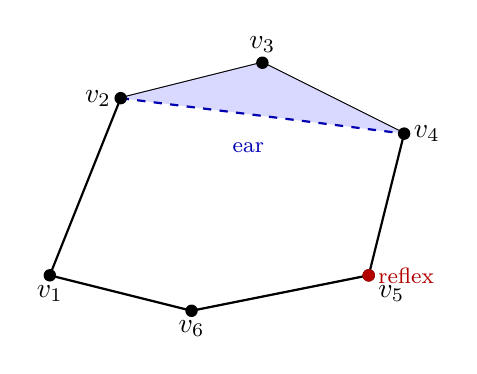
\begin{tikzpicture}[scale=0.9]
  \coordinate (A) at (0,0);
  \coordinate (B) at (1,2.5);
  \coordinate (C) at (3,3);
  \coordinate (D) at (5,2);
  \coordinate (E) at (4.5,0);
  \coordinate (F) at (2,-0.5);
  \draw[thick] (A)--(B)--(C)--(D)--(E)--(F)--cycle;
  \fill[blue!15] (B)--(C)--(D)--cycle;
  \draw[thick,blue!70!black,dashed] (B)--(D);
  \foreach \v/\name/\pos in {A/$v_1$/below,B/$v_2$/left,C/$v_3$/above,D/$v_4$/right,E/$v_5$/below right,F/$v_6$/below} {
    \fill (\v) circle (2.5pt) node[\pos] {\name};
  }
  \node[blue!70!black] at (2.8,1.8) {\footnotesize ear};
  \fill[red!70!black] (E) circle (2.5pt);
  \node[red!70!black,right] at (E) {\footnotesize reflex};
\end{tikzpicture}
\caption{Ear clipping: vertex $v_3$ is an ``ear'' since triangle $(v_2, v_3, v_4)$ is entirely inside the polygon and contains no other vertices.}
\label{fig:ear_clipping}
\end{figure}
